\section{Experiments}
\label{sec:experiments}

\subsection{Data Sets}

We evaluated our implementations of various algorithms on 3 diverse datasets. The feature sets include real numbers, intergers and categorical values. The datasets are randomly split into training sets $80\%$ and
testing sets $20\%$. For multi-class data sets we do one-vs-all (OVA)
classifiers. For approximations that has reasonable run time, we will perform
cross-validation to select parameters for prior, which may have profound
impact on the result as suggested by~\cite{Asuncion2009smoothing}. Details of each dataset can found in Table~\ref{tb:datasets}.

\begin{table}
\begin{tabular}{| c | c |  c | c | c |}
  \hline
  Datasets & \# training instances & \# test instances & \# features & class-wise split\\
  \hline
  Yeast & 1500 & 917 & 103 & (14 classes) \\
  \hline
  Spambase & 3680 & 921 & 57 & 39\% vs. 61\% \\
  \hline
  Heart Diseases & 216 & 54 & 13 & 44\% vs. 56\% \\
  \hline
\end{tabular}

\caption{Datasets information}
\label{tb:datasets}
\end{table}

\subsection{Results}

We compare classification accuracy and run-time of different algorithms. Results are shown in Fig~\ref{fig:results}.

The top graph shows the comparision of different algorithm's classification accuracy. First, we observe that the sampling algorithm outperforms all variational-based approaches on all datasets. However, this does not conclude we should always choose sampling algorithm for better accuracy. Sampling based algorithm suffers when the dimensionality of the data is high. Second, we observe that Delta method performs worse than other three algorithms on all three datasets. This does not necessarily show that the delta method is less accurate. First, the delta method is very sensitive to the step size parameter. We might have not yet tuned that parameter optimally. Second, the delta method takes a long time to converge. We might not have waited long enough for it to converge.

The bottom graph shows the comparison of different algorithm's runtime. We conducted our experiemnts on different platforms since we expected the difference among different algorithms to be siginificant and a rough comparison would be sufficient. We observe that sampling is indeed slower than traditional variational algorithms, which confirms our conventional wisdom. We also observe that the delta method is siginificantly slower than the other three approaches which confirms the complexity of this algorithm.

\begin{figure}[t]
\centering
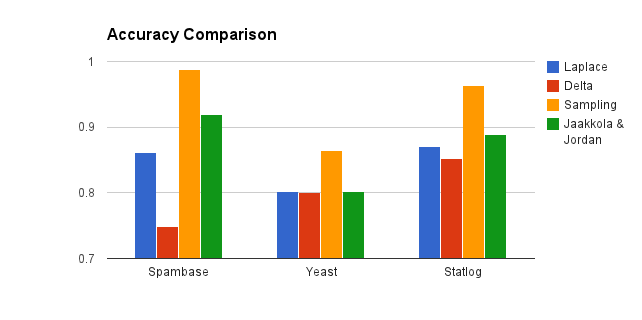
\includegraphics[height=7.0cm]{results/accuracy_comp.png}
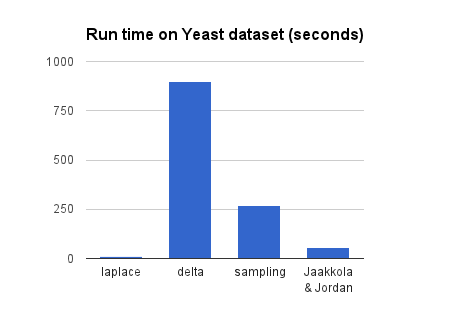
\includegraphics[height=8.0cm]{results/speed_comp.png}

\caption{\small Experiment results; {\bf Top:} Classification accuracy of all algorithms on
four datasets. {\bf Bottom:} Runtime for each algorithm on Yeast dataset. }
\label{fig:results}
\end{figure}

\subsubsection{MCMC based converging chains}
Our Kolmogorov Smirnove based Gibbs sampling strategy that we described in
section~\ref{sec:MCMCmethod} consistently to same set of parameters.
Figure~\ref{fig:MCMCconverge} is a plot of the iterations of the two
independent Markov chains for estimation on the spambase dataset. 
The X-axix of the figure represents the number of
iteration in sampling and Y-axis is the loglikelihood of the regression model.
As we can see both the chains converge to the same log-likelihood value and the
chains seem to be stable after convergence. Compare this to the markov chain
produce via uniform distribution based sampling methos in
figure~\ref{fig:uniformSamplerChain}. the chain in this case is not stable and
keeps oscillating between different log-likelihood states. 
 

\begin{figure}[hbt]
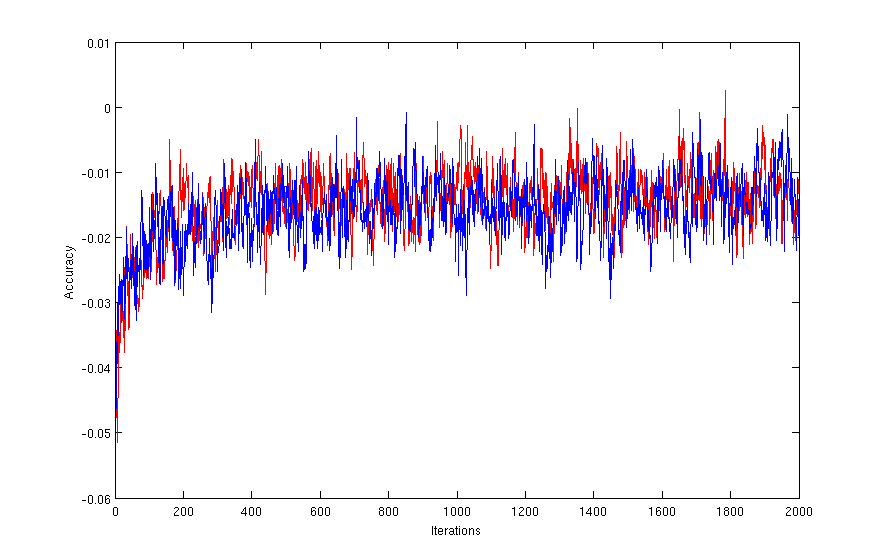
\includegraphics[width=1\textwidth]{results/KSsampleChain.png}
\caption{Two Markov chains (red and blue) converge on the same set of
parameters on the spambase dataset. The
X-axis is the number of iterations and Y-axis is the loglikelihood.}
\label{fig:MCMCconverge}
\end{figure}
